% Need pgf to compile, may not compile with
%  current stable version, in which case :
%  - download last pgf build from
%    http://media.texample.net/pgf/builds/pgfCVS2009-03-10_TDS.zip
%  - dezip it in /usr/local/share/texmf
%  - run "sudo texhash"

\documentclass[a4paper]{easychair}
%\documentclass[a4paper]{article}

\usepackage{graphicx}
\usepackage{color}
\usepackage{times}
\usepackage{amsmath}
\usepackage{amsthm}
\usepackage{amssymb}

\renewcommand{\O}[1]{\mathrm{O}\left(#1\right)}
\newcommand{\IGNORE}[1]{}
\newcommand{\N}{\mathbb{N}}
\newcommand{\Z}{\mathbb{Z}}
\newcommand{\C}{\mathbb{C}}
\newcommand{\m}{\mbox}

\everymath{\displaystyle}

%\RequirePackage{tikz}
\usepackage{tikz}
\usetikzlibrary{shapes}
\usetikzlibrary{arrows,decorations.pathmorphing,backgrounds,positioning,fit}
\tikzset{terminal node/.style={ellipse, draw,
    rounded corners, shade, top color=white, bottom 
    color=blue!50!black!20, draw=blue!40!black!60, thick}}
\tikzset{mdd node/.style={terminal node, rectangle split, rectangle split horizontal, rectangle split parts=#1}}
\tikzset{regular edge/.style={draw=blue!40!black!60, thick}}
\tikzset{outgoing edge/.style={regular edge, very thin}}
\tikzset{comment/.style={blue!95}}
\tikzset{diagram background/.style={fill=blue!2,rounded corners=0.5cm}}

\usepackage{algorithm}
\usepackage[noend]{algorithmic}
\renewcommand{\algorithmiccomment}[1]{  // \emph{#1}}
\newcommand{\BLANK}{\STATE \vspace{-0.6em}}

\newcommand{\edge}[2]{\langle #1, #2 \rangle}
\newcommand{\val}[1]{#1{\rm .val}}
\newcommand{\node}[1]{#1{\rm .node}}
\newcommand{\level}[1]{#1{\rm .level}}

\newtheorem{definition}{Definition}
\newtheorem{theorem}{Theorem}
\newtheorem{lemma}{Lemma}
\newtheorem{example}{Example}

\setlength{\headheight}{15pt}

%========================================================

\title{Model Checking with Edge Valued Decision Diagrams}
\titlerunning{Model Checking with Edge-valued Decision Diagrams}

\author{Pierre Roux, 
\'{E}cole Normale Sup\'{e}rieure de Lyon, France.
\url{pierre.roux@ens-lyon.fr}
\and
Radu I. Siminiceanu, 
National Institute of Aerospace, Hampton, Virginia, USA.
\url{radu@nianet.org}
}
\authorrunning{Roux \& Siminiceanu}
\cfoot{} % To avoid page numbers

%=======================================================

\begin{document}

%\pagestyle{plain}

\maketitle

\thispagestyle{empty}

\begin{abstract}
We describe an algebra of Edge-Valued Decision Diagrams (EVMDDs) to 
encode arithmetic functions and its implementation in a model checking 
library.
%
We provide efficient algorithms for manipulating EVMDDs and review
the theoretical time complexity of these algorithms for all basic 
arithmetic and relational operators. We also demonstrate that the time 
complexity of the generic recursive algorithm for applying a binary 
operator on EVMDDs is no worse than that of Multi-Terminal Decision 
Diagrams.

We have implemented a new symbolic model checker with the intention to 
represent in one formalism the best techniques available at the moment 
across a spectrum of existing tools.
Compared to the CUDD package, our tool is several orders of magnitude faster.


\end{abstract}

%=======================================================
\section{Introduction}

Binary decision diagrams (BDD)~\cite{Bryant1986} have 
revolutionized the reachability analysis and model checking technology. 
% 
Arithmetic decision diagrams~\cite{Somenzi1993}, also called Multi-Terminal
Binary Decision Diagrams (MTBDD)~\cite{Clarke1995} are the 
natural extension of regular BDDs to arithmetic functions. They take 
advantage of the symbolic encoding scheme of BDDs, but functions with 
large co-domains do not usually have a very compact representation 
because there are less chances for suffixes to be shared.

Edge-valued decision diagrams have been previously 
introduced, but only scarcely used. An early version, the edge valued binary 
decision diagrams (EVBDD)~\cite{Lai1992}, is particularly useful 
when representing both arithmetic and logic functions, which is the case 
for discrete state model checking. However, EVBDD have only been applied 
to rather obscure applications: computing the probability spectrum and 
the Reed-Muller spectrum of (pseudo)-Boolean functions. 

Binary Moment Diagrams~\cite{Bryant1994} were designed to overcome the 
limitations of BDDs/EVBDDs when encoding multiplier functions.
However, their efficiency seems to be limited only to this particular 
type of functions.
%
A new canonization rule for edge-valued decision diagrams enabling them 
to encode functions in $\Z \cup \{+\infty\}$ was introduced 
in~\cite{FMCAD2002} along with EVMDDs, an extension to multi-way diagrams 
(MDD)~\cite{Kam1998}, but, again, this was applied to a very specific 
task, of finding minimum length counterexamples for safety properties. 
Later, EVMDDs have been also used for partial reachability analysis.

In this paper we first present a theoretical comparison between EVMDDs 
and MTMDDs for building the transition relation of discrete state 
systems before dealing with an implementation in a model checker along 
with state-of-the-art algorithms for state space construction.

%===========================================================
\section{Background}

%-----------------------------------------------------------
\subsection{Discrete-state Systems}\label{sec:DSS}

A discrete--state model is a triple $(S,S_0,T)$, where
the discrete set $S$ is the \emph{potential state space} of the model;
the set $S_0\subseteq S$ contains the \emph{initial states};
and $T : S\rightarrow 2^{S}$ is the \emph{transition function}
specifying which states can be reached from a given state in one step, 
which we extend to sets: $T(X) = \bigcup_{i\in X}T(i)$.
We consider structured systems modeled as a collection of $K$~\emph{submodels}.
A (global) system state $i$ is then a $K$-tuple $(i_{K},\ldots,i_{1})$,
where~$i_{k}$ is the \emph{local state} for submodel~$k$,
for $K \!\geq\! k\! \geq\! 1$, and
$S$ is given by $ S_K \times \cdots \times  S_{1}$,
the cross--product of $K$ local state spaces $ S_k$,
which we identify with $\{0,\ldots,n_k\!-\!1\}$ since
we assume that $S$ is finite.
The \emph{(reachable) state space} $R \subseteq S$ is the
smallest set containing $S_0$ and closed with respect to $T$,
i.e.
$R = S_0 \cup T(S_0) \cup
T(T(S_0) \cup \cdots = T^{\ast}(S_0).$
Thus, $R$ is the least fixpoint of function $X \mapsto S_0 \cup T(X)$.

%-----------------------------------------------------------
\subsection{Decision Diagrams}

We discuss the extension of BDDs to integer variables,
i.e., multi--valued decision diagrams (MDDs) \cite{Kam1998}.
We assume that the variables along any path from the root must follow 
the order $x_K, \ldots, x_1$. Ordered MDDs can be either \emph{reduced} 
(no duplicate nodes and no node with all edges pointing to the same 
node, but edges possibly spanning multiple levels) or 
\emph{quasi--reduced} (no duplicate nodes, and all edges spanning 
exactly one level), either form being \emph{canonical}.

%=======================================================
\section{EVMDDs}

%-------------------------------------------------------
\begin{definition}{\rm  \label{DEF:evmdd}}
An \emph{EVMDD} on a group $(G, *)$, is a pair $A = \edge{v}{n}$,
where $v \in G$ is the edge \emph{value} also denoted as $\val{A}$ 
and $n$ is a \emph{node} also denoted $\node{A}$. 

A \emph{node} $n$ is either the unique terminal node $\langle 0, e 
\rangle$ where $e$ is the identity element of $G$, or a pair $\langle k, 
p \rangle$ where $1 \leq k \leq K$ and $p$ is an array of edges of size 
$n_k$ (cardinality of $S_k$). 
The first element of the pair will be denoted $\level{n}$ and, when relevant,
the $i$-th element in the array will be denoted by $n[i]$.
\end{definition}

\begin{definition}{\rm  \label{DEF:evmdd-function}}
For a node $n$ with $\level{n} = k$ and 
$\left(i_k,\ldots, i_1\right) \in S_k \times \cdots \times S_1$,
we define $n(i_k,\ldots, i_1)$ as $\val{n[i_k]}$ if $\level{\node{n[i_k]}} = 0$ and
$\val{n[i_k]}*\node{n[i_k]}(i_{\level{\node{n[i_k]}}},\ldots, i_1)$ otherwise.


The \emph{function encoded} by an EVMDD $A$,
$f : S \rightarrow G, (i_K,\ldots, i_1) \mapsto \val{A} * \node{A}(i_{\level{\node{A}}},\ldots, i_1)$
is the repetitive  application of law $*$  on the edge values along the path
from the root to the terminal node,
corresponding to arcs $i_k$, for $K\geq k \geq 1$:
\end{definition}

\begin{definition}\label{definition-reduced}
A \emph{canonical node} is either the terminal node or a node $n$ such 
that $\val{n[0]} = e$.

A \emph{canonical} EVMDD contains only canonical nodes.

\end{definition}

It can be proved that any function $f$ has a unique
canonical EVMDD representation~\cite{FMCAD2002}.

Examples of graph representations of EVMDDs are given in 
Figure~\ref{figure-reduced}.

\begin{figure}[htbp]
  \centering
  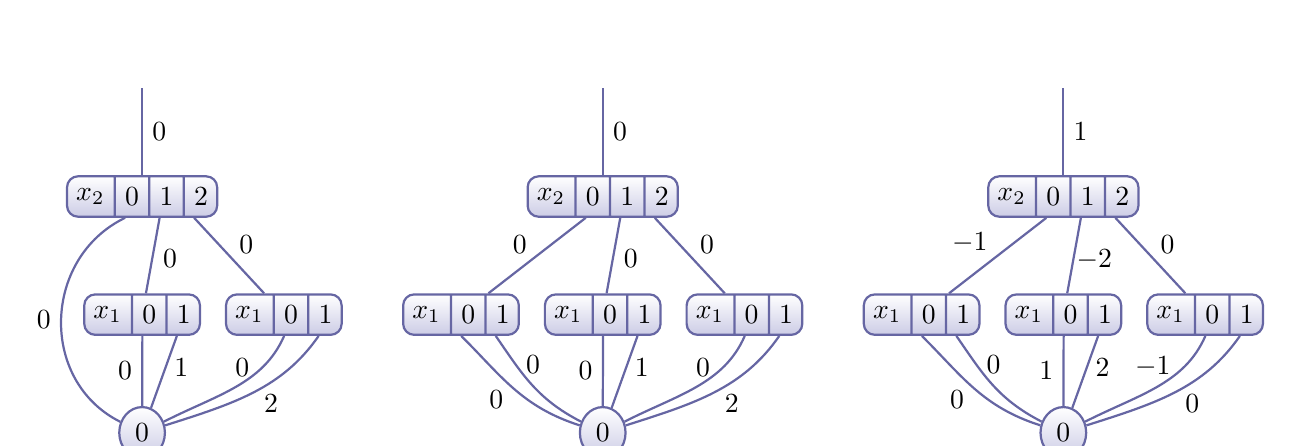
\begin{tikzpicture}
  [xscale=1.8, yscale=1.5, auto]
  \begin{scope}
%    \node [comment, xshift=-0.5cm]   at ( 0, 3) {$A$};

    \node                 (top)      at ( 0, 3) {};
    \node [mdd node=4]    (l2n0)     at ( 0, 2) {$x_2$\nodepart{two}0\nodepart{three}1\nodepart{four}2};
    \node [mdd node=3]    (l1n1)     at ( 0, 1) {$x_1$\nodepart{two}0\nodepart{three}1};
    \node [mdd node=3]    (l1n2)     at ( 1, 1) {$x_1$\nodepart{two}0\nodepart{three}1};
    \node [terminal node] (terminal) at ( 0, 0) {0};
    
    \draw [regular edge]  (top)                      to                   node                   {$0$} (l2n0);
    \draw [regular edge]  (l2n0.two   |- l2n0.south) to [out=-150,in=150] node [swap]            {$0$} (terminal);
    \draw [regular edge]  (l2n0.three |- l2n0.south) to                   node [yshift=2mm]      {$0$} (l1n1);
    \draw [regular edge]  (l2n0.four  |- l2n0.south) to                   node [yshift=-1mm]     {$0$} (l1n2);
    \draw [regular edge]  (l1n1.two   |- l1n1.south) to                   node [swap]            {$0$} (terminal);
    \draw [regular edge]  (l1n1.three |- l1n1.south) to                   node [yshift=3mm]      {$1$} (terminal);
    \draw [regular edge]  (l1n2.two   |- l1n1.south) to [out=-110,in=30]  node [swap,xshift=3mm] {$0$} (terminal);
    \draw [regular edge]  (l1n2.three |- l1n1.south) to [out=-120,in=20]  node [yshift=1mm]      {$2$} (terminal);
  \end{scope}
  
  \begin{scope}[xshift=3.25cm]
%    \node [comment, xshift=-0.5cm]   at ( 0, 3) {$A$};

    \node                 (top)      at ( 0, 3) {};
    \node [mdd node=4]    (l2n0)     at ( 0, 2) {$x_2$\nodepart{two}0\nodepart{three}1\nodepart{four}2};
    \node [mdd node=3]    (l1n0)     at (-1, 1) {$x_1$\nodepart{two}0\nodepart{three}1};
    \node [mdd node=3]    (l1n1)     at ( 0, 1) {$x_1$\nodepart{two}0\nodepart{three}1};
    \node [mdd node=3]    (l1n2)     at ( 1, 1) {$x_1$\nodepart{two}0\nodepart{three}1};
    \node [terminal node] (terminal) at ( 0, 0) {0};
    
    \draw [regular edge]  (top)                      to                   node                    {$0$} (l2n0);
    \draw [regular edge]  (l2n0.two   |- l2n0.south) to                   node [swap,yshift=-1mm] {$0$} (l1n0);
    \draw [regular edge]  (l2n0.three |- l2n0.south) to                   node [yshift=2mm]       {$0$} (l1n1);
    \draw [regular edge]  (l2n0.four  |- l2n0.south) to                   node [yshift=-1mm]      {$0$} (l1n2);
    \draw [regular edge]  (l1n0.two   |- l1n1.south) to [out=-50,in=160]  node [swap,yshift=1mm]  {$0$} (terminal);
    \draw [regular edge]  (l1n0.three |- l1n1.south) to [out=-60,in=150]  node [xshift=-2mm]      {$0$} (terminal);
    \draw [regular edge]  (l1n1.two   |- l1n1.south) to                   node [swap]             {$0$} (terminal);
    \draw [regular edge]  (l1n1.three |- l1n1.south) to                   node [yshift=3mm]       {$1$} (terminal);
    \draw [regular edge]  (l1n2.two   |- l1n1.south) to [out=-110,in=30]  node [swap,xshift=3mm]  {$0$} (terminal);
    \draw [regular edge]  (l1n2.three |- l1n1.south) to [out=-120,in=20]  node [yshift=1mm]       {$2$} (terminal);
  \end{scope}
  
  \begin{scope}[xshift=6.5cm]
%    \node [comment, xshift=-0.5cm]   at ( 0, 3) {$A$};

    \node                 (top)      at ( 0, 3) {};
    \node [mdd node=4]    (l2n0)     at ( 0, 2) {$x_2$\nodepart{two}0\nodepart{three}1\nodepart{four}2};
    \node [mdd node=3]    (l1n0)     at (-1, 1) {$x_1$\nodepart{two}0\nodepart{three}1};
    \node [mdd node=3]    (l1n1)     at ( 0, 1) {$x_1$\nodepart{two}0\nodepart{three}1};
    \node [mdd node=3]    (l1n2)     at ( 1, 1) {$x_1$\nodepart{two}0\nodepart{three}1};
    \node [terminal node] (terminal) at ( 0, 0) {0};
    
    \draw [regular edge]  (top)                      to                   node                          { $1$} (l2n0);
    \draw [regular edge]  (l2n0.two   |- l2n0.south) to                   node [swap,yshift=-1mm]       {$-1$} (l1n0);
    \draw [regular edge]  (l2n0.three |- l2n0.south) to                   node [xshift=-1mm,yshift=2mm] {$-2$} (l1n1);
    \draw [regular edge]  (l2n0.four  |- l2n0.south) to                   node [yshift=-1mm]            { $0$} (l1n2);
    \draw [regular edge]  (l1n0.two   |- l1n1.south) to [out=-50,in=160]  node [swap,yshift=1mm]        { $0$} (terminal);
    \draw [regular edge]  (l1n0.three |- l1n1.south) to [out=-60,in=150]  node [xshift=-2mm]            { $0$} (terminal);
    \draw [regular edge]  (l1n1.two   |- l1n1.south) to                   node [swap]                   { $1$} (terminal);
    \draw [regular edge]  (l1n1.three |- l1n1.south) to                   node [yshift=3mm]             { $2$} (terminal);
    \draw [regular edge]  (l1n2.two   |- l1n1.south) to [out=-110,in=30]  node [swap,xshift=3mm]        {$-1$} (terminal);
    \draw [regular edge]  (l1n2.three |- l1n1.south) to [out=-120,in=20]  node [yshift=1mm]             { $0$} (terminal);
  \end{scope}
\end{tikzpicture}
  
  \caption{EVMDDs on $(\Z, +)$ representing the same function
   $f:\{0, 1, 2\}\times\{0, 1\}\rightarrow\Z, (x_2, x_1)\mapsto x_2\cdot x_1$.
   The leftmost EVMDD is reduced while the others are quasi--reduced.
   The rightmost EVMDD is not canonical.}
\label{figure-reduced}
\end{figure}

%-------------------------------------------------------
EVMDDs can be used when even the algebraic structure $G$ is not a group.
For example, \cite{FMCAD2002} offers a canonization rule for $\N\cup \{+\infty\}$.
Also, $(\Z, \times)$ that can be handled with the canonization rule
``${\rm gcd}\{\val{n[i]}\;|\; i \in S_{\level{n}}\} = 1$ and
$(\val{n[0]},\ldots, \val{n[n_{\level{n}}]}) \geq_{\rm lex} 0$''.

%=======================================================
\section{EVMDDs compared to MTMDDs}

MTBDDs are commonly used in model checking to build the transition 
relation of discrete-state systems. In this section we show that EVMDDs 
are at least as suited to that purpose and oftentimes significantly 
better. In the following, we choose, without loss of generality, $(G, *) = (\Z, +)$.

%-------------------------------------------------------
\subsection{Space Complexity}

\begin{theorem}\label{th:spacecomplexity}
  \label{theorem-evmdd-smaller-than-add}
  For any function $f$, the number of nodes of the EVMDD representing $f$
  is at most the number of nodes of the MTMDD representing the same function 
$f$.\footnote{All proofs and algorithms are given in a technical report~\cite{Roux10}, to appear.}
\end{theorem}

%-------------------------------------------------------
\subsection{Time complexity%
  \label{subsection-time-complexity}}

Section 2 of~\cite{Clarke1995} gives an algorithm to compute any
binary operation on BDDs. The \emph{apply} algorithm can be
easily generalized to MDDs for any
$n$-ary operator $\square_n$. It computes its result in time
$\O{\prod_{i=1}^n |f_i|}$, where $|f_i|$ is the size (in nodes) of the MTMDD representing
operand $i$.

Section 2.2 of~\cite{Lai1996} gives the equivalent \emph{apply} algorithm for
edge-valued decision diagrams.

\begin{theorem}
\label{th:rec-calls}
The number of recursive calls of the generic \emph{apply} algorithm for MTMDDs
is equal to that for EVMDDs representing the same function~\cite{Lai1996}.
\end{theorem}

Hence, EVMDD computations are at least not worse than the MTMDD 
counterpart. However, particular operators $\square_n$ may enable much 
better algorithms on EVMDDs. Below is a synopsis of the basic algorithms to
manipulate EVMDDs.
%.......................................................
\begin{itemize}
\addtolength{\itemsep}{-0.5ex}
\item Addition of constant ($f + c$): $\O{1}$.
\item Multiplication with scalar ($f \times c$): $\O{|f|}$~\cite{Lai1996}.
\item Addition ($f + g$): $\O{|f|\;|g|}$~\cite{Lai1996}.
%Algorithm~\ref{algorithm-sum} offers a simple upper bound: $|f+g| \leq |f| \; |g|$.
\item Remainder and Euclidean Division: $\O{|f|c}$.
\item Minimum and Maximum: $O(|f|)$.
\item Relational Operator with constant ($f < c$): not better in the worst case,\\
but in practice the complexity can be improved, by using min and max.
\item Relational Operators ($f < g$): can be computed as $(f-g < 0)$.
\end{itemize}

\subsection{Multiplication}

As stated in~\cite{Lai1996},
the result of a multiplication can have an EVMDD
representation of exponential size in terms of the operands.
For example, let $S$ be $\{0, 1\}^K$, $f : (x_K,\ldots, x_1) \mapsto \sum_{k=2}^K x_k2^{k-2}$
and $g : (x_K,\ldots, x_1) \mapsto x_1$, $f$ and $g$ both have an EVMDD representation with $K+1$ nodes
whereas $f{\cdot}g$ has $2^K$ nodes.
Therefore, we cannot expect to find an algorithm with better worst-case
complexity. However, the following equation, coming from the decomposition
of $\edge{v}{n}$ in $v + \edge{0}{n}$ and $\edge{v'}{n'}$ in $v' + \edge{0}{n'}$
$$
\edge{v}{n}\times\edge{v'}{n'} = vv'+v\edge{0}{n'}+v'\edge{0}{n}+\edge{0}{n}\times\edge{0}{n'}
$$
suggests an alternative algorithm.

The first product is an integer multiplication done in constant time.
The next two are multiplications by a constant done in $\O{|f|}$ and $\O{|g|}$, respectively.
The last one is done through recursive calls.
The first addition takes constant time, the second one
takes $\O{|f|\;|g|}$ and produce a result of size at most $|f|\;|g|$,
hence a cost of $\O{|f|\;|g|\;|fg|}$ for the last addition.
The recursive function is called $\O{|f|\;|g|}$ times, hence a final complexity
of $\O{|f|^2\;|g|^2\;|fg|}$.

Although we were unable to theoretically compare this algorithm to
the generic \emph{apply} algorithm, it seems to perform
far better on practical cases.

%=======================================================
\section{Implementation}

{\small
\begin{table}[htb]
  \begin{center}
    \m{\hspace{-2mm}\begin{tabular}{|r||r||r|r|r|}
      \hline
      \multicolumn{1}{|l||}{\footnotesize Model} & \multicolumn{1}{l||}{\footnotesize Reachable} & {\footnotesize CUDD} & {\footnotesize SMART} & {\footnotesize EVMDD} \\
      \multicolumn{1}{|l||}{\footnotesize size}  & \multicolumn{1}{l||}{\footnotesize states}  & {\footnotesize (in s)} & {\footnotesize (in s)} & {\footnotesize (in s)} \\
      \hline
      \multicolumn{5}{|l|}{Dining philosophers}\\
      \hline
      100 & $4\times10^{62}$ &   11.42 &    1.49 &    0.03 \\
      200 & $2\times10^{125}$ & 3054.69 &    3.03 &    0.07 \\
      15000 & $2\times10^{9404}$ &   --- &   --- &  195.29 \\
      \hline
      \multicolumn{5}{|l|}{Round robin mutual exclusion protocol}\\
      \hline
      40 & $9\times10^{13}$ &    4.44 &    0.44 &    0.08 \\
      100 & $2\times10^{32}$ &   --- &    2.84 &    1.17 \\
      200 & $7\times10^{62}$ &   --- &   20.02 &    9.14 \\
      \hline
      \multicolumn{5}{|l|}{Slotted ring protocol}\\
      \hline
      10 & $8\times10^{9}$ &    1.16 &    0.19 &    0.01 \\
      20 & $2\times10^{20}$ &   --- &    0.71 &    0.04 \\
      200 & $8\times10^{211}$ &   --- &  412.27 &   25.97 \\
      \hline
    \end{tabular}
    \hspace{2mm}
    \begin{tabular}{|r||r||r|r|r|r|}
      \hline
      \multicolumn{1}{|l||}{\footnotesize Model} & \multicolumn{1}{l||}{\footnotesize Reachable} & {\footnotesize CUDD} & {\footnotesize SMART} & {\footnotesize EVMDD} \\
      \multicolumn{1}{|l||}{\footnotesize size}  & \multicolumn{1}{l||}{\footnotesize states}  & {\footnotesize (in s)} & {\footnotesize (in s)} & {\footnotesize (in s)} \\
      \hline
      \multicolumn{5}{|l|}{Kanban assembly line}\\
      \hline
      15 & $4\times10^{10}$ &   80.43 &    3.41 &    0.01 \\
      20 & $8\times10^{11}$ & 2071.58 &    8.23 &    0.02 \\
      400 & $6\times10^{25}$ &   --- &   --- &   74.89 \\
      \hline
      \multicolumn{5}{|l|}{Knights problem}\\
      \hline
      5 & $6\times10^{7}$ & 1024.42 &    5.29 &    0.27 \\
      7 & $1\times10^{15}$ &   --- &  167.41 &    3.46 \\
      9 & $8\times10^{24}$ &   --- &   --- &   32.20 \\
      \hline
      \multicolumn{5}{|l|}{Randomized leader election protocol}\\
      \hline
      6 & $2\times10^{6}$ &   4.22 &    8.42 &    0.86 \\
      9 & $5\times10^{9}$ &   --- &  954.81 &   18.89 \\
      11 & $9\times10^{11}$ &   --- &   --- &  109.25 \\
      \hline
    \end{tabular}}
%\vspace*{3mm}
    \caption{Execution times for building state space using our library or CUDD (``---'' means ``$>1$hour'').}
    \label{table-results}
  \end{center}
\end{table}
}
\vspace*{-5mm}


\IGNORE{
{\small
\begin{table}[htb]
  \begin{center}
    \m{\hspace{-2mm}\begin{tabular}{|r||r||r|r|r|}
      \hline
      \multicolumn{1}{|l||}{\footnotesize Model} & \multicolumn{1}{l||}{\footnotesize Reachable} & {\footnotesize CUDD} & {\footnotesize SMART} & {\footnotesize EVMDD} \\
      \multicolumn{1}{|l||}{\footnotesize size}  & \multicolumn{1}{l||}{\footnotesize states}  & {\footnotesize (in s)} & {\footnotesize (in s)} & {\footnotesize (in s)} \\
      \hline
      \multicolumn{5}{|l|}{Dining philosophers}\\
      \hline
      100 & $4\times10^{62}$ &    5.65 & 0.75 &    0.02 \\
      200 & $2\times10^{125}$ & 1566.73 & 1.55 &   0.06 \\
%      1000 & $9\times10^{626}$ &   --- &    1.10 \\
%      5000 & $6\times10^{3134}$ &   --- &   20.48 \\
      10000 & $4\times10^{6269}$ &   --- & 195.68 &  73.10 \\
%      16000 & $2\times10^{10031}$ &   --- &  196.84 \\
      \hline
      \multicolumn{5}{|l|}{Round robin mutual exclusion protocol}\\
      \hline
%      20 & $4\times10^{7}$ &    0.47 &    0.04 \\
      40 & $9\times10^{13}$ &    5.30 &    0.28 & 0.11 \\
%      60 & $1\times10^{20}$ &   15.59 &    1.54 \\
      100 & $2\times10^{32}$ &  599.16 &    2.20 & 1.56 \\
      200 & $7\times10^{62}$ &   --- &   15.94 & 10.75 \\
      \hline
      \multicolumn{5}{|l|}{Slotted ring protocol}\\
      \hline
      10 & $8\times10^{9}$    &    1.13 &    0.11 & 0.01 \\
%      15 & $1\times10^{15}$   &   13.00 &    0.03 \\
      20 & $2\times10^{20}$   & 1937.35 & 0.48 &    0.05 \\
%      100 & $2\times10^{105}$ &   --- &    3.74 \\
%      200 & $8\times10^{211}$ &   --- &   29.73 \\
%      300 & $3\times10^{318}$ &   --- &  111.29 \\
      500 & $5\times10^{531}$ &   --- & --- & 738.70 \\
      \hline
    \end{tabular}
    \hspace{2mm}
    \begin{tabular}{|r||r||r|r|r|r|}
      \hline
      \multicolumn{1}{|l||}{\footnotesize Model} & \multicolumn{1}{l||}{\footnotesize Reachable} & {\footnotesize CUDD} & {\footnotesize SMART} & {\footnotesize EVMDD} \\
      \multicolumn{1}{|l||}{\footnotesize size}  & \multicolumn{1}{l||}{\footnotesize states}  & {\footnotesize (in s)} & {\footnotesize (in s)} & {\footnotesize (in s)} \\
      \hline
      \multicolumn{5}{|l|}{Kanban assembly line}\\
      \hline
%      10 & $1\times10^{9}$   &    0.84 &    0.01 \\
      15 & $4\times10^{10}$  &   90.20 & 1.82 &    0.00 \\
      20 & $8\times10^{11}$  &  922.08 & 4.67 &    0.01 \\
%      100 & $1\times10^{19}$ &   --- &    3.25 \\
%      200 & $3\times10^{22}$ &   --- &   32.31 \\
      400 & $6\times10^{25}$ &   --- & --- & 112.78 \\
      \hline
      \multicolumn{5}{|l|}{Knights problem}\\
      \hline
      5 & $6\times10^{7}$  &  985.54 & 4.59 &   0.88 \\
      7 & $1\times10^{15}$ &   --- & 157.57 &    12.18 \\
      9 & $8\times10^{24}$ &   --- & --- &   66.27 \\
      \hline
      \multicolumn{5}{|l|}{Randomized leader election protocol}\\
      \hline
%      5 & $1\times10^{5}$   &    0.90 &    0.32 \\
      6 & $2\times10^{6}$   &    4.48 & 6.74 &    1.38 \\
%      7 & $2\times10^{7}$   &   23.87 &    3.69 \\
%      8 & $3\times10^{8}$   &  176.16 &   10.04 \\
      9 & $5\times10^{9}$   &  857.79 & 818.74 &   30.11 \\
%      10 & $6\times10^{10}$ &   ---   &   85.54 \\
      11 & $9\times10^{11}$ &   ---   & --- &  465.21 \\
      \hline
    \end{tabular}}
%\vspace*{3mm}
    \caption{Execution times for building state space using our library vs. CUDD (``---'' means ``$>1$hour'').}
    \label{table-results}
  \end{center}
\end{table}
}
\vspace*{-5mm}
}

Symbolic model checkers, such as (Nu)SMV or SAL,
are based on the library CUDD\cite{CUDD} which offers an efficient
implementation of BDDs and MTBDDs.
Our goal was to implement a new symbolic model checking library featuring
EVMDDs for the transition relation construction and saturation\cite{Saturation2001}
for state space generation. We also developed a basic
model checking front-end to test the library and compare it to CUDD.
Binaries and source code for both the EVMDD library and the model checker are available
at \url{http://research.nianet.org/~radu/evmdd/}.

%-------------------------------------------------------
\subsection{Encoding the Transition Relation}

We represent the transition relation $T$ as a disjunction of events
which is well suited for globally--asynchronous locally--synchronous systems,
where each event encodes some local transition.
To avoid the expensive coding of lot of identities,
we use the \emph{full-identity reduction} from~\cite{Ciardo2005}.

%-------------------------------------------------------
\subsection{State Space Construction}

For state space construction, we use the Saturation 
algorithm~\cite{Saturation2001} instead of the classical breadth first 
search exploration. This heuristic often gives spectacular improvements 
when building the state spaces of globally--asynchronous 
locally--synchronous systems. This is certainly the major source of 
improvement of our implementation over existing BDD libraries.

%We chose to merge all events $e$ with same topmost affected level in the same MDD. The cost of the 
%unions slows down the generation of the transition relation but generally makes the state space 
%construction up to several times faster.

%-------------------------------------------------------
\subsection{Experimental Results}

Our new tool comprises 7K~lines of ANSI-C code for the library 
and 4K~lines for the simple model checker that provides a common 
interface to both our library and CUDD. Table~\ref{table-results} shows 
execution times for building the state space on a suite of classical models. 
Programs to generate all models can be found in the 
\texttt{examples} folder of our source code distribution.

We collected the results on a Linux machine with 
Intel~Core~2 processor, 1.2GHz, 1.5GB of memory.

Note that using other existing tools, such as NuSMV or SAL on these 
models, we get execution times of the same order of magnitude as with 
the CUDD interface of our tool.

Compared to the first implementation of saturation 
algorithm~\cite{Saturation2001} in the tool SMART, our new 
implementation is always several (up to a few dozens) times faster. This 
is due to both the encoding of the transition relation and our simple C 
implementation in comparison to the object-oriented C++ version.

%=======================================================
\section{Conclusions and Future Work}

We have studied the advantages of the EVMDD data structure
over the widely used MTBDDs for the construction
of transition relations of finite state systems
and implemented them in a library, along with
state-of-the-art algorithms for state space generation.
We obtained execution times several orders of magnitude faster
than the CUDD library and classical algorithms,
with a reduced memory usage enabling to handle extremely large systems.
Future work should focus primarily on integrating our library
into the SAL model checker.

Our results show that symbolic model checking remains an efficient 
technique for analyzing globally--asynchronous locally--synchronous 
systems and significant improvements are still possible.

%=======================================================
\bibliographystyle{abbrv}
\bibliography{evmdd}

\IGNORE{
\begin{appendix}

\section{Proofs}

\noindent\textbf{Theorem 1}.
  For any function $f$, the number of nodes of the EVMDD representing $f$
  is at most the number of nodes of the MTMDD representing the same function $f$.

  \begin{figure}[htbp]
    \centering
        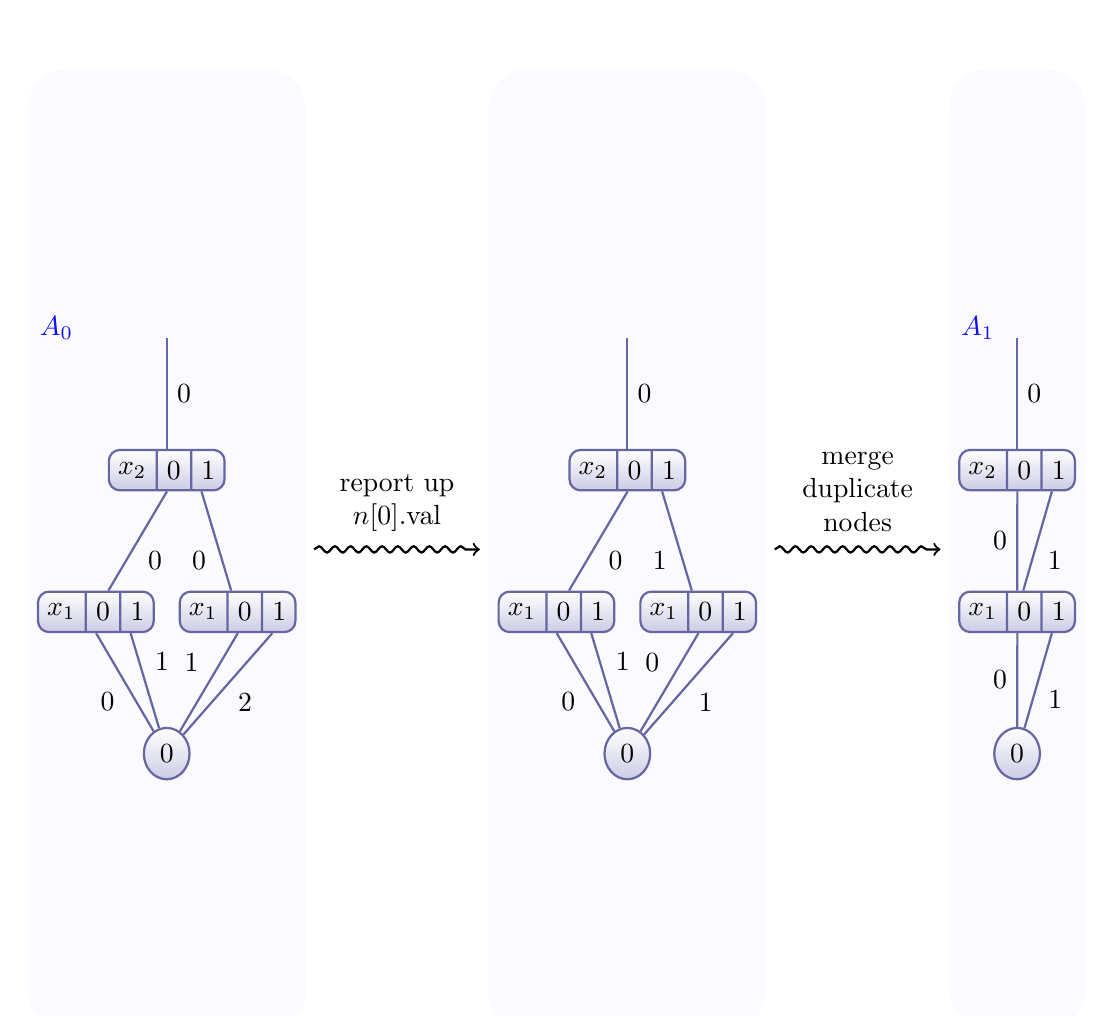
\begin{tikzpicture}
      [xscale=0.9, yscale=1.8, auto]
      \begin{scope}
        \node [comment, xshift=-0.5cm]   at (-1, 3) {$A_0$};

        \node                 (top)      at ( 0, 3) {};
        \node [mdd node=3]    (l2n0)     at ( 0, 2) {$x_2$\nodepart{two}0\nodepart{three}1};
        \node [mdd node=3]    (l1n0)     at (-1, 1) {$x_1$\nodepart{two}0\nodepart{three}1};
        \node [mdd node=3]    (l1n1)     at ( 1, 1) {$x_1$\nodepart{two}0\nodepart{three}1};
        \node [terminal node] (terminal) at ( 0, 0) {0};

        \draw [regular edge]  (top)                      to node        {0} (l2n0);
        \draw [regular edge]  (l2n0.two   |- l2n0.south) to node        {0} (l1n0);
        \draw [regular edge]  (l2n0.three |- l2n0.south) to node [swap] {0} (l1n1);
        \draw [regular edge]  (l1n0.two   |- l1n0.south) to node [swap] {0} (terminal);
        \draw [regular edge]  (l1n0.three |- l1n0.south) to node        {1} (terminal);
        \draw [regular edge]  (l1n1.two   |- l1n1.south) to node [swap] {1} (terminal);
        \draw [regular edge]  (l1n1.three |- l1n1.south) to node        {2} (terminal);
      \end{scope}

      \begin{scope}[xshift=6.5cm]
        \node                 (top')      at ( 0, 3) {};
        \node [mdd node=3]    (l2n0')     at ( 0, 2) {$x_2$\nodepart{two}0\nodepart{three}1};
        \node [mdd node=3]    (l1n0')     at (-1, 1) {$x_1$\nodepart{two}0\nodepart{three}1};
        \node [mdd node=3]    (l1n1')     at ( 1, 1) {$x_1$\nodepart{two}0\nodepart{three}1};
        \node [terminal node] (terminal') at ( 0, 0) {0};

        \draw [regular edge]  (top')                       to node        {0} (l2n0');
        \draw [regular edge]  (l2n0'.two   |- l2n0'.south) to node        {0} (l1n0');
        \draw [regular edge]  (l2n0'.three |- l2n0'.south) to node [swap] {1} (l1n1');
        \draw [regular edge]  (l1n0'.two   |- l1n0'.south) to node [swap] {0} (terminal');
        \draw [regular edge]  (l1n0'.three |- l1n0'.south) to node        {1} (terminal');
        \draw [regular edge]  (l1n1'.two   |- l1n1'.south) to node [swap] {0} (terminal');
        \draw [regular edge]  (l1n1'.three |- l1n1'.south) to node        {1} (terminal');
      \end{scope}

      \begin{scope}[xshift=12cm]
        \node [comment, xshift=-0.5cm]     at ( 0, 3) {$A_1$};

        \node                 (top'')      at ( 0, 3) {};
        \node [mdd node=3]    (l2n0'')     at ( 0, 2) {$x_2$\nodepart{two}0\nodepart{three}1};
        \node [mdd node=3]    (l1n0'')     at ( 0, 1) {$x_1$\nodepart{two}0\nodepart{three}1};
        \node [terminal node] (terminal'') at ( 0, 0) {0};

        \draw [regular edge]  (top'')                        to node        {0} (l2n0'');
        \draw [regular edge]  (l2n0''.two   |- l2n0''.south) to node [swap] {0} (l1n0'');
        \draw [regular edge]  (l2n0''.three |- l2n0''.south) to node        {1} (l1n0'');
        \draw [regular edge]  (l1n0''.two   |- l1n0''.south) to node [swap] {0} (terminal'');
        \draw [regular edge]  (l1n0''.three |- l1n0''.south) to node        {1} (terminal'');
      \end{scope}

      \begin{pgfonlayer}{background}
        \node [yscale=2] (r1) [diagram background, fit=(top)(l2n0)(l1n0)(l1n1)(terminal)] {};
        \node [yscale=2] (r2) [diagram background, fit=(top')(l2n0')(l1n0')(l1n1')(terminal')] {};
        \node [yscale=2] (r3) [diagram background, fit=(top'')(l2n0'')(l1n0'')(terminal'')] {};
      \end{pgfonlayer}

      \draw [shorten >=1mm,-to,thick,decorate,
      decoration={snake,amplitude=.4mm,segment length=2mm,
        pre=moveto,pre length=1mm,post length=2mm}]
      (r1) -- (r2) node [above=1mm,midway,text width=2cm,text centered]
      {report up $\val{n[0]}$};
      \draw [shorten >=1mm,-to,thick,decorate,
      decoration={snake,amplitude=.4mm,segment length=2mm,
        pre=moveto,pre length=1mm,post length=2mm}]
      (r2) -- (r3) node [above=1mm,midway,text width=2cm,text centered]
      {merge duplicate nodes};
    \end{tikzpicture}
    
    \caption{Constructing EVMDD $A_1$ (right) from EVMDD $A_0$ (left)}
    \label{figure-A0-to-A1}
  \end{figure}

\begin{proof}
  Let $A$ be the MTMDD representing $f$. From $A$ we construct the EVMDD (not in canonical form) $A_0$ by replacing each edge from level $1$ to a terminal with value $v$ with an edge with value $v$ to the unique terminal node $0$ and associating value $0$ to all other edges (see Figure~\ref{figure-A-to-A0} for an example).
  \begin{figure}[htbp]
    \centering
        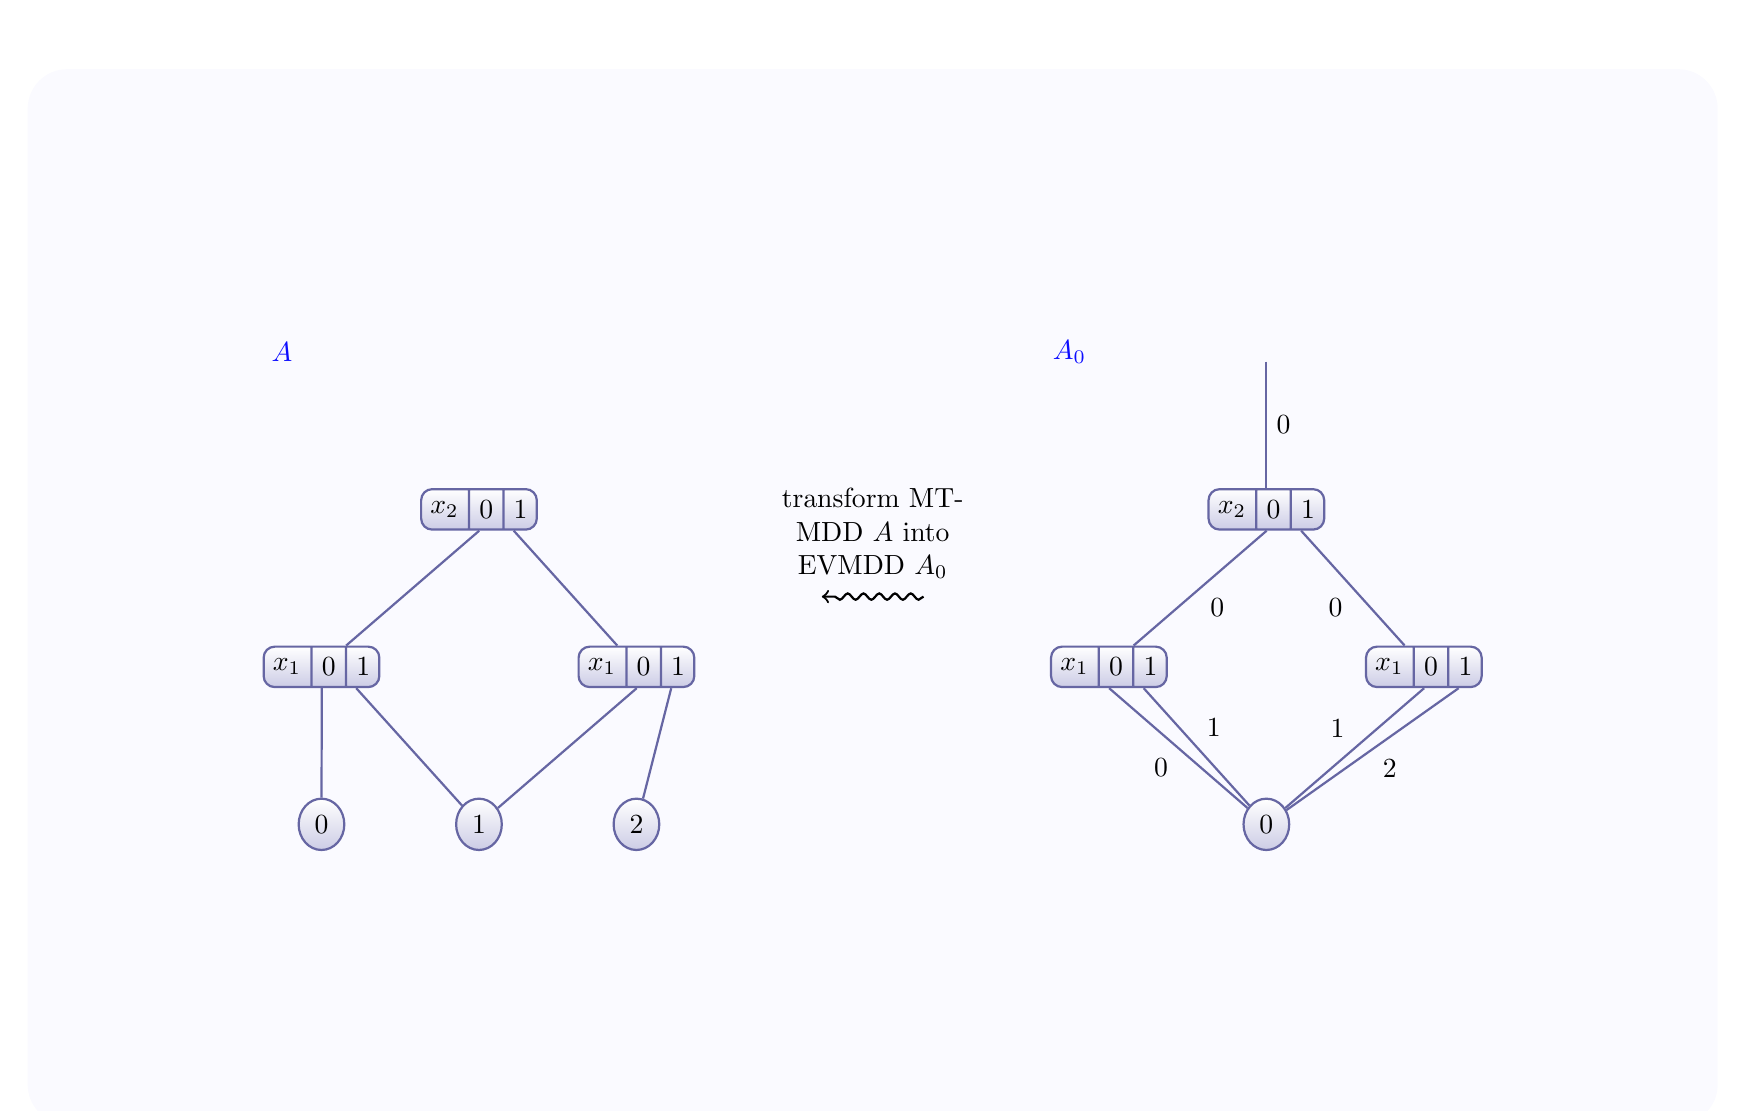
\begin{tikzpicture}
      [scale=2, auto]
      \begin{scope}
        \node [comment, xshift=-0.5cm]    at (-1, 3) {$A$};

        \node                 (top)       at ( 0, 3) {};
        \node [mdd node=3]    (l2n0)      at ( 0, 2) {$x_2$\nodepart{two}0\nodepart{three}1};
        \node [mdd node=3]    (l1n0)      at (-1, 1) {$x_1$\nodepart{two}0\nodepart{three}1};
        \node [mdd node=3]    (l1n1)      at ( 1, 1) {$x_1$\nodepart{two}0\nodepart{three}1};
        \node [terminal node] (terminal0) at (-1, 0) {0};
        \node [terminal node] (terminal1) at ( 0, 0) {1};
        \node [terminal node] (terminal2) at ( 1, 0) {2};

        \draw [regular edge]  (l2n0.two   |- l2n0.south) to (l1n0);
        \draw [regular edge]  (l2n0.three |- l2n0.south) to (l1n1);
        \draw [regular edge]  (l1n0.two   |- l1n0.south) to (terminal0);
        \draw [regular edge]  (l1n0.three |- l1n0.south) to (terminal1);
        \draw [regular edge]  (l1n1.two   |- l1n1.south) to (terminal1);
        \draw [regular edge]  (l1n1.three |- l1n1.south) to (terminal2);
      \end{scope}

      \begin{scope}[xshift=5cm]
        \node [comment, xshift=-0.5cm]    at (-1, 3) {$A_0$};

        \node                 (top')      at ( 0, 3) {};
        \node [mdd node=3]    (l2n0')     at ( 0, 2) {$x_2$\nodepart{two}0\nodepart{three}1};
        \node [mdd node=3]    (l1n0')     at (-1, 1) {$x_1$\nodepart{two}0\nodepart{three}1};
        \node [mdd node=3]    (l1n1')     at ( 1, 1) {$x_1$\nodepart{two}0\nodepart{three}1};
        \node [terminal node] (terminal') at ( 0, 0) {0};


        \draw [regular edge]  (top')                       to node        {0} (l2n0');
        \draw [regular edge]  (l2n0'.two   |- l2n0'.south) to node        {0} (l1n0');
        \draw [regular edge]  (l2n0'.three |- l2n0'.south) to node [swap] {0} (l1n1');
        \draw [regular edge]  (l1n0'.two   |- l1n0'.south) to node [swap] {0} (terminal');
        \draw [regular edge]  (l1n0'.three |- l1n0'.south) to node        {1} (terminal');
        \draw [regular edge]  (l1n1'.two   |- l1n1'.south) to node [swap] {1} (terminal');
        \draw [regular edge]  (l1n1'.three |- l1n1'.south) to node        {2} (terminal');
      \end{scope}

      \begin{pgfonlayer}{background}
        \node [scale=2] (r1) [diagram background, fit=(top)(l2n0)(l1n0)(l1n1)(terminal0)(terminal1)(terminal2)] {};
        \node [scale=2] (r2) [diagram background, fit=(top')(l2n0')(l1n0')(l1n1')(terminal')] {};
      \end{pgfonlayer}

      \draw [shorten >=1mm,-to,thick,decorate,
      decoration={snake,amplitude=.4mm,segment length=2mm,
        pre=moveto,pre length=1mm,post length=2mm}]
      (r1) -- (r2) node [above=1mm,midway,text width=3cm,text centered]
      {transform MTMDD $A$ into EVMDD $A_0$};
    \end{tikzpicture}

    \caption{Building the EVMDD $A_0$ (right) from MTMDD $A$ (left)}
    \label{figure-A-to-A0}
  \end{figure}
  Then, we iteratively compute the EVMDD $A_k$, for each $k$ from $1$ to $n$, through the following process:
  \begin{itemize}
  \item for each node $n$ at level $k$, subtract $\val{n[0]}$ from all outgoing edges and add this value to all incoming edges;
  \item merge all duplicate nodes at level $k$ (by duplicate nodes we mean two nodes having edges $x_i$ holding same value and pointing to same children for each $i$ in the range of variable $x_k$).
  \end{itemize}
  See Figure~\ref{figure-A0-to-A1} for an example.

To prove that $A_k$ and $A$ represent the same function, it is 
sufficient to see that $A$ and $A_0$ represent the same function and that 
the iterative transformation preserves the sum of values on any path $(i_K, \ldots, i_1)$ from 
the root of the diagram to the unique terminal node (plus the value
of the root's incoming edge)
$$
\val{A_k}+\node{A_k}(i_K, \ldots, i_1) = \val{A_{k-1}}+\node{A_{k-1}}(i_K, \ldots, i_1)
$$

Since $A_K$ is in canonical form and since for each $k$, the number of nodes of 
$A_k$ is at most the number of nodes of $A_{k-1}$, 
we can conclude that the size of an EVMDD is never larger than that of the corresponding MTMDD.
\end{proof}

\noindent\textbf{Theorem 2}.
The number of recursive calls of the generic \emph{apply} algorithm is 
the same for MTMDDs and for EVMDDs representing the same function~\cite{Lai1996}.

  We show the proof for the unary version of the algorithm.
  Proofs for other versions are similar, only a bit more verbose.

\begin{lemma}\label{lemma-n-k-1}

Two paths $(i_K, \ldots, i_{k+1})$ and $(j_K, \ldots, j_{k+1})$ lead to 
the same node in $A$
$$
\node{A}[i_K, \ldots, i_{k+1}] = \node{A}[j_K, \ldots, j_{k+1}]
$$
if and only if they lead to the same node in $A_{k-1}$
$$
\node{A_{k-1}}[i_K, \ldots, i_{k+1}] = A_{k-1}[j_K, \ldots, j_{k+1}]
$$
\end{lemma}

\begin{lemma}\label{lemma-n-k}
  Two paths $(i_K, \ldots, i_{k+1})$ and $(j_K, \ldots, j_{k+1})$ lead to the same node in $A_K$ with the same value
$$
\begin{array}{ll}
&\node{A_K}[i_K, \ldots, i_{k+1}] = \node{A_K}[j_K, \ldots, j_{k+1}]\\
\;\;\;\m{and}\;\;\;&
\node{A_K}(i_K, \ldots, i_{k+1}) = \node{A_K}(j_K, \ldots, j_{k+1})
\end{array}
$$
if and only if they lead to the same node in $A_k$ with the same value
$$
\begin{array}{ll}
&\node{A_k}[i_K, \ldots, i_{k+1}] = \node{A_k}[j_K, \ldots, j_{k+1}]\\
\;\;\;\m{and}\;\;\;&
\node{A_k}(i_K, \ldots, i_{k+1}) = \node{A_k}(j_K, \ldots, j_{k+1})
\end{array}
$$
\end{lemma}


\begin{proof}

If we do not take into consideration the caches, the two algorithms are 
obviously equivalent so what we need to prove is that a cache hit occurs 
in the EVMDD \emph{apply} algorithm with diagram $A_K$ if and only if it 
occurs in the MTMDD algorithm with diagram $A$. In other words, we have 
to prove for every two paths $(i_K, \ldots, i_{k+1})$ and $(j_K, \ldots, 
j_{k+1})$ that they lead to the same node in $A$ $$ \node{A}[i_K, 
\ldots, i_{k+1}] = \node{A}[j_K, \ldots, j_{k+1}] $$ if and only if they 
reach the same node in $A_K$ with the same value: $$ \begin{array}{ll} 
&\node{A_K}[i_K, \ldots, i_{k+1}] = \node{A_K}[j_K, \ldots, j_{k+1}]\\ 
\;\;\;\m{and}\;\;\;& \node{A_K}(i_K, \ldots, i_{k+1}) = \node{A_K}(j_K, 
\ldots, j_{k+1}) \end{array} $$

Therefore, from lemmas \ref{lemma-n-k-1} and \ref{lemma-n-k} it remains to prove 
that two paths $(i_K, \ldots, i_{k+1})$ and $(j_K, \ldots, j_{k+1})$ lead to 
the same node in $A_{k-1}$
\begin{equation}
\label{eqn-k-1}
\node{A_{k-1}}[i_K, \ldots, i_{k+1}] = \node{A_{k-1}}[j_K, \ldots, j_{k+1}]
\end{equation}
if and only if they reach the same node in $A_k$ with the same value:
\begin{equation}
\label{eqn-k}
\begin{array}{ll}
&\node{A_k}[i_K, \ldots, i_{k+1}] = \node{A_k}[j_K, \ldots, j_{k+1}]\\
\;\;\;\m{and}\;\;\;&
\node{A_k}(i_K, \ldots, i_{k+1}) = \node{A_k}(j_K, \ldots, j_{k+1})
\end{array}
\end{equation}

\begin{itemize}

\item Let us prove that (\ref{eqn-k-1}) implies (\ref{eqn-k}).
The first part of (\ref{eqn-k}) is obvious: if two paths lead to the same node before
merging, this still holds after merging. Second part is slightly more complex.
Indeed, $\node{A_k}(i_K, \ldots, i_{k+1})$ is just the value attached to edge $i_{k+1}$ of node
$\node{A_k}[i_K, \ldots, i_{k+2}]$ since all other edges hold value $0$. This value
is the one reported up when constructing $A_k$ from $A_{k-1}$ for 
node $\node{A_k}[i_K, \ldots, i_{k+1}] = \node{A_k}[j_K, \ldots, j_{k+1}]$ so it is the
same for $\node{A_k}(j_K, \ldots, j_{k+1})$, which is the second part of (\ref{eqn-k}).

\item In the other direction: (\ref{eqn-k}) implies (\ref{eqn-k-1}). \\
If (\ref{eqn-k}) holds then $\node{A_{k-1}}[i_K, \ldots, i_{k+1}]$ and
$\node{A_{k-1}}[j_K,\ldots, j_{k+1}]$ are identical (for if they were not, then (\ref{eqn-k})
does not hold on $A_k$ computed from $A_{k-1}$). Hence (\ref{eqn-k-1}), since
$A_{k-1}$ doesn't contain any duplicate at level $k$.

\end{itemize}
\end{proof}

%----------------------------------------
\section{Algorithms}

Following algorithms are for quasi-reduced DDs.
Although they are slightly more verbose, versions for reduced diagrams can be easily derived.

\begin{algorithm}[htbp]
  \caption{Computes any binary operation $\square_2$ on EVMDDs $\edge{v}{n}$ and $\edge{v'}{n'}$}
  \label{algorithm-generic}
  \begin{algorithmic}
    \item[apply($\square_2$ : edge $*$ edge $\rightarrow$ edge, $\edge{v}{n}$ : edge, $\edge{v'}{n'}$ : edge) : edge]
    \STATE $k \gets \level{n}$ \COMMENT{$= \level{n'}$ since EVMDDs are quasi-reduced}
    \BLANK
    \STATE \COMMENT{base case}
    \IF{$k = 0$}
      \RETURN $\edge{v \,\square_2\, v'}{t}$ \COMMENT{$t$ is the unique terminal node}
    \ENDIF
    \BLANK
    \STATE \COMMENT{lookup in cache}
    \IF{CacheFind($\square_2$, $\edge{v}{n}$, $\edge{v'}{n'}$, $\edge{m}{r}$)}
      \RETURN $\edge{m}{r}$
    \ENDIF
    \BLANK
    \STATE $r \gets$ NewNode($k$)
    \FOR{$i = 0$ \textbf{to} $n_k-1$}
      \STATE $r[i] \gets$ apply($\square_2$, $\edge{v+\val{n[i]}}{\node{n[i]}}$, $\edge{v'+\val{n'[i]}}{\node{n'[i]}}$)
    \ENDFOR
    \STATE $m \gets \val{r[0]}$
    \FOR{$i = 0$ \textbf{to} $n_k-1$}
      \STATE $\val{r[i]} \gets \val{r[i]} - m$
    \ENDFOR 
    \BLANK
    \STATE \COMMENT{check if a node identical to $r$ already exists}
    \STATE $r \gets$ FindOrAdd($r$)
    \BLANK
    \STATE \COMMENT{save result in cache}
    \STATE CacheInsert($\square_2$, $\edge{v}{n}$, $\edge{v'}{n'}$, $\edge{m}{r}$)
    \BLANK
    \RETURN $\edge{m}{r}$
  \end{algorithmic}
\end{algorithm}

\begin{algorithm}[htbp]
  \caption{Computes product of EVMDDs $\edge{v}{n}$ and $\edge{v'}{n'}$}
  \label{algorithm-product}
  \begin{algorithmic}
    \item[times($\edge{v}{n}$ : edge, $\edge{v'}{n'}$ : edge) : edge]
    \STATE $k \gets \level{n}$ \COMMENT{$= \level{n'}$ since EVMDDs are quasi-reduced}
    \BLANK
    \STATE \COMMENT{base case}
    \IF{$k = 0$}
      \RETURN $\edge{v\times v'}{t}$ \COMMENT{$t$ is the unique terminal node}
    \ENDIF
    \BLANK
    \STATE \COMMENT{lookup in cache}
    \IF{CacheFind($\times$, $\edge{0}{n}$, $\edge{0}{n'}$, $r$)}
      \RETURN plusc(plus(plus(timesc($\edge{0}{n}$, $v'$), timesc($\edge{0}{n'}$, $v$)), r), $v\times v'$)
    \ENDIF
    \BLANK
    \STATE $r \gets$ NewNode($k$)
    \FOR{$i = 0$ \textbf{to} $n_k-1$}
      \STATE $r[i] \gets$ times($n[i]$, $n'[i]$)
    \ENDFOR
    \BLANK
    \STATE \COMMENT{check if a node identical to $r$ already exists}
    \STATE $r \gets$ FindOrAdd($r$)
    \BLANK
    \STATE \COMMENT{save result in cache}
    \STATE CacheInsert($\times$, $\edge{v}{n}$, $\edge{v'}{n'}$, $\edge{m}{r}$)
    \BLANK
    \RETURN plusc(plus(plus(timesc($\edge{0}{n}$, $v'$), timesc($\edge{0}{n'}$, $v$)), r), $v\times v'$)
  \end{algorithmic}
\end{algorithm}

\begin{algorithm}[htbp]
  \caption{Computes $\edge{v}{n} < c$ for EVMDD $\edge{v}{n}$ and integer $c$}
  \label{algorithm-lt}
  \begin{algorithmic}
    \item[lt($\edge{v}{n}$ : edge, $c$ : int) : edge]
    \STATE $k \gets \level{n}$
    \BLANK
    \STATE \COMMENT{base cases}
    \IF{$c-v \leq {\rm min}(n)$}
      \RETURN $\edge{0}{t}$ \COMMENT{$t$ is the unique terminal node}
    \ENDIF
    \IF{$c-v > {\rm max}(n)$}
      \RETURN $\edge{1}{t}$ \COMMENT{$t$ is the unique terminal node}
    \ENDIF
    \BLANK
    \STATE \COMMENT{lookup in cache}
    \IF{CacheFind($<$, $\edge{0}{n}$, $c-v$, $\edge{m}{r}$)}
      \RETURN $\edge{m}{r}$
    \ENDIF
    \BLANK
    \STATE $r \gets$ NewNode($k$)
    \FOR{$i = 0$ \textbf{to} $n_k-1$}
      \STATE $r[i] \gets$ lt($n[i]$, $c-v$)
    \ENDFOR
    \STATE $m \gets \val{r[0]}$
    \FOR{$i = 0$ \textbf{to} $n_k-1$}
      \STATE $\val{r[i]} \gets \val{r[i]}-m$
    \ENDFOR
    \BLANK
    \STATE \COMMENT{check if a node identical to $r$ already exists}
    \STATE $r \gets$ FindOrAdd($r$)
    \BLANK
    \STATE \COMMENT{save result in cache}
    \STATE CacheInsert($<$, $\edge{0}{n}$, $c-v$, $\edge{m}{r}$)
    \BLANK
    \RETURN $\edge{m}{r}$
  \end{algorithmic}
\end{algorithm}

\end{appendix}
}
\end{document}
